\documentclass[a4paper]{article}

\usepackage[english]{babel}
\usepackage[utf8]{inputenc}
\usepackage{amsmath}
\usepackage{graphicx}
\usepackage[colorinlistoftodos]{todonotes}
\usepackage{enumerate}
\usepackage{eqnarray}

\textheight=10in
\textwidth=6.9in
\topmargin=0.0in
\headheight=-0.3in
\headsep=-0.3in
\leftmargin=-0.2in
\rightmargin=-0.4in
\oddsidemargin=-0.3in
\evensidemargin=-0.5in
\parindent=0.0in

\pagestyle{empty}

\def\ss{\displaystyle\sum}
\def\ii{\displaystyle\int}
\def\lb{\left(}
\def\rb{\right)}
\def\lB{\left[}
\def\rB{\right]}
\def\E{\mathrm{E}}
\def\Var{\mathrm{Var}}
\def\Cov{\mathrm{Cov}}
\def\Pr{\mathrm{Pr}}
\def\erf{\mathrm{erf}}
\def\erfinv{\mathrm{erfinv}}
\linespread{1.2}

\title{FINA4140 HW3}

\author{You}

\date{\today}

\begin{document}
\begin{enumerate}
\item Problem 1
\begin{enumerate}
\item 
\begin {enumerate}
\item Since $W^{(1)}$ and $W^{(2)}$ are white noise processes, we have:\\
$W^{(1)}(s)-W^{(1)}(t)\sim N(0,s-t)$ and $W^{(2)}(s)-W^{(2)}(t)\sim N(0,s-t)$ for all $s,t$ with $s>t$\\
Hence, $\rho\lb W^{(1)}(s)-W^{(1)}(t)\rb\sim N(0,\rho^2(s-t))$\\
$\sqrt{1-\rho^2}\lb W^{(2)}(s)-W^{(2)}(t)\rb\sim N(0,(1-\rho^2)(s-t))$\\
For all $s,t$ with $s>t$, $W(s)-W(t)=\rho\lb W^{(1)}(s)-W^{(1)}(t)\rb+\sqrt{1-\rho^2}\lb W^{(2)}(s)-W^{(2)}(t)\rb$\\
Since $W^{(1)}$ and $W^{(2)}$ are independent, summing the two independent normal distributions gives:\\
$W(s)-W(t)\sim N(0,\rho^2(s-t)+(1-\rho^2)(s-t))=N(0,s-t)$\\
Therefore, $W$ is a white noise process.\\

\item For all $s,t$ with $s>t$, \\define $X=W(s)-W(t), X_1=W^{(1)}(s)-W^{(1)}(t),X_2=W^{(2)}(s)-W^{(2)}(t)$\\
Since $W$, $W^{(1)}$ and $W^{(2)}$ are white noise processes,\\
$\E\lB X\rB=\E\lB X_1\rB=\E\lB X_2\rB=0,\Var(X)=\Var(X_1)=\Var(X_2)=s-t$\\
Also, since $W^{(1)}$ and $W^{(2)}$ are independent, $\Cov(X_1, X_2)=0$\\
$\E\lB X_1 X_2\rB=\Cov(X_1, X_2)+E\lB X_1\rB E\lB X_2\rB=0+0=0$\\
$X=W(s)-W(t)=\lb\rho W^{(1)}(s)+\sqrt{1-\rho^2}W^{(2)}(s)\rb-\lb\rho W^{(1)}(t)+\sqrt{1-\rho^2}W^{(2)}(t)\rb\\
=\rho\lb W^{(1)}(s)-W^{(1)}(t)\rb+\sqrt{1-\rho^2}\lb W^{(2)}(s)-W^{(2)}(t)\rb=\rho X_1+\sqrt{1-\rho^2}X_2$\\
$\Cov(X,X_1)=\E\lB XX_1\rB-\E\lB X\rB\E\lB X_1\rB=\E\lB XX_1\rB=\E\lB \rho X_1^2+\sqrt{1-\rho^2}X_2X_1\rB\\
=\rho\E\lB X_1^2\rB+\sqrt{1-\rho^2}\E\lB X_2X_1\rB=\rho\E\lB X_1^2\rB\\
=\rho\Var(X_1)+\rho\E\lB X_1\rB^2=\rho\Var(X_1)=\rho(s-t)$\\
Therefore, the correlation between $W$ and $W^{(1)}$\\
$=\frac{\Cov(X,X_1)}{\sqrt{\Var(X)\Var(X_1)}}=\frac{\rho(s-t)}{s-t}=\rho$\\

\item Correlation between $W$ and $W^{(2)}$ is $\sqrt{1-\rho^2}$\\
\end{enumerate}
\item Since $t_{i+1}>t>t_i$, $t_{i+1}-t_i>t-t_i>0$, $1=\frac{t_{i+1}-t_i}{t_{i+1}-t_i}>\frac{t-t_i}{t_{i+1}-t_i}=\lambda>0$\\
As $\lambda(1-\lambda)>0$, we can set $\alpha=\sqrt{\lambda(1-\lambda)(t_{i+1}-t_i)}$ and
\[ W(t)=(1-\lambda)W(t_i)+\lambda W(t_{i+1})+\alpha\omega \]
where $\omega\sim N(0,1)$ independent from $W(t_i)$ and $W(t_{i+1})$\\
i.e. $\E\lB\alpha\omega\rB=0$, $\Var(\alpha\omega)=\alpha^2$, $\Cov(W(t_{i+1})-W(t_i),\omega)=0$\\
Now verify the statistical properties of $W(t)-W(t_i)$ and $W(t_{i+1})-W(t)$ :

\begin{enumerate}
\item $\E\lB W(t)-W(t_i)\rB=\E\lB\lambda(W(t_{i+1})-W(t_i))+\alpha\omega\rB=\lambda\E\lB W(t_{i+1})-W(t_i)\rB+\E\lB\alpha\omega\rB=0\\
\E\lB W(t_{i+1})-W(t)\rB=\E\lB(1-\lambda)(W(t_{i+1})-W(t_i))-\alpha\omega\rB=(1-\lambda)\E\lB W(t_{i+1})-W(t_i)\rB-\E\lB\alpha\omega\rB=0$

\item 
$\Var(W(t)-W(t_i))=\Var(\lambda(W(t_{i+1})-W(t_i))+\alpha\omega)\\
=\Var(\lambda(W(t_{i+1})-W(t_i)))+\Var(\alpha\omega)+2\Cov(\lambda(W(t_{i+1})-W(t_i)),\alpha\omega)\\
=\lambda^2\Var(W(t_{i+1})-W(t_i))+\alpha^2+2\lambda\alpha\Cov(W(t_{i+1})-W(t_i),\omega)\\
=\lambda^2(t_{i+1}-t_i)+\lambda(1-\lambda)(t_{i+1}-t_i)+0=\lambda(t_{i+1}-t_i)=t-t_i$\\
$\Var(W(t_{i+1})-W(t))=\Var((1-\lambda)(W(t_{i+1})-W(t_i))-\alpha\omega)\\
=\Var((1-\lambda)(W(t_{i+1})-W(t_i)))+\Var(\alpha\omega)-2\Cov((1-\lambda)(W(t_{i+1})-W(t_i)),\alpha\omega)\\
=(1-\lambda)^2\Var(W(t_{i+1})-W(t_i))+\alpha^2-2(1-\lambda)\alpha\Cov(W(t_{i+1})-W(t_i),\omega)\\
=(1-\lambda)^2(t_{i+1}-t_i)+\lambda(1-\lambda)(t_{i+1}-t_i)-0=(1-\lambda)(t_{i+1}-t_i)=t_{i+1}-t$

\pagebreak

\item
Since $W(t_{i+1})-W(t_i)\sim N(0,t_{i+1}-t_i)$,\\
$E\lB(W(t_{i+1})-W(t_i))\rB=0,\E\lB(W(t_{i+1})-W(t_i))^2\rB=t_{i+1}-t_i$\\
Also, as $\omega\sim N(0,1)$ is independent from $W(t_i)$ and $W(t_{i+1})$, we have\\
$\E\lB(W(t_{i+1})-W(t_i))\omega\rB=\Cov(W(t_{i+1})-W(t_i),\omega)=0$\\
Since $\E\lB W(t)-W(t_i)\rB=\E\lB W(t_{i+1})-W(t)\rB=0$,\\
$\Cov(W(t)-W(t_i),W(t_{i+1})-W(t))=\E\lB(W(t)-W(t_i))(W(t_{i+1})-W(t))\rB\\
=\E\lB(\lambda(W(t_{i+1})-W(t_i))+\alpha\omega)((1-\lambda)(W(t_{i+1})-W(t_i))-\alpha\omega)\rB\\
=\E\lB\lambda(1-\lambda)(W(t_{i+1})-W(t_i))^2+(1-2\lambda)(W(t_{i+1})-W(t_i))\alpha\omega-\alpha^2\omega^2\rB\\
=\lambda(1-\lambda)\E\lB(W(t_{i+1})-W(t_i))^2\rB+(1-2\lambda)\alpha\E\lB(W(t_{i+1})-W(t_i))\omega\rB-\alpha^2\E\lB\omega^2\rB\\
=\lambda(1-\lambda)(t_{i+1}-t_i)+0-\lambda(1-\lambda)(t_{i+1}-t_i)=0$\\
Hence we have shown that $W(t)-W(t_i)$ and $W(t_{i+1})-W(t)$ are uncorrelated.\\
$W(t)-W(t_i)$ is normally distributed, since $W(t)-W(t_i)=\lambda(W(t_{i+1})-W(t_i))+\alpha\omega$, where $\lambda(W(t_{i+1})-W(t_i))$ and $\alpha\omega$ are normally distributed and independent. Sum of independent normally distributed random variables is also normally distributed. The same holds for $W(t_{i+1})-W(t)$.\\
Since $W(t)-W(t_i)$ and $W(t_{i+1})-W(t)$ are normally distributed, zero correlation implies that they are independent.
\end{enumerate}
Thus, we have shown that $W(t)-W(t_i)$ and $W(t_{i+1})-W(t)$ have the correct statistical properties.

\end{enumerate}

\pagebreak

\item Problem 2
\begin{enumerate}
\item
$\ii_0^t \,dW(\tau)=\lim_{N\rightarrow\infty}\sum_{i=0}^{N-1}\lb W(t_{i+1})-W(t_i)\rb=\lim_{N\rightarrow\infty}\lb W(t_N)-W(t_0)\rb=W(t)-W(0)$, where $t_i=\frac{i}{N}t$\\
$\ii_0^t\tau\,dW(\tau)=\lim_{N\rightarrow\infty}\sum_{i=0}^{N-1}t_i\lb W(t_{i+1})-W(t_i)\rb\\
=\lim_{N\rightarrow\infty}\sum_{i=0}^{N-1}\lb t_{i+1}W(t_{i+1})-t_iW(t_i)\rb-\lim_{N\rightarrow\infty}\sum_{i=0}^{N-1}\lb t_{i+1}W(t_{i+1})-t_iW(t_{i+1})\rb\\
=t_NW(t_N)-t_0W(0)-\lim_{N\rightarrow\infty}\sum_{i=0}^{N-1}(t_{i+1}-t_i) W(t_{i+1})=tW(t)-\ii_0^t W(\tau)\,d\tau$, where $t_i=\frac{i}{N}t$

\item
Referring to Excel,\\
$N=1000, t=1$, hence we define $t_i=\frac{i}{1000}$ and $W_i$ calculated by:\\
$W(0)=0$, $W(t_{i+1})=W(t_i)+\frac{\omega_i}{\sqrt{1000}}$ for $0\leq i<1000$\\
where $\omega_i\sim N(0,1)$ is independent of $\{t_i\}$\\
Then, $W(t_i)$ approximates a white noise path.\\
$\ii_0^1 W\,dW$ is approximated by $\displaystyle\sum_{i=0}^{999}W(t_i)(W(t_{i+1})-W(t_i))$\\
According to our simulation, $\displaystyle\sum_{i=0}^{999}W(t_i)(W(t_{i+1})-W(t_i))=-0.27790$\\
$W(1)=-0.67581$, $\frac{1}{2}W(1)^2=0.22836$, $\frac{1}{2}W(1)^2-\frac{1}{2}=-0.27164$\\
Therefore, $\frac{1}{2}W(1)^2-\frac{1}{2}$ is closer.

\item
$N=1000, t=1$, hence we define $t_i=\frac{i}{1000}$\\
Using Euler-Maruyama method, $X(t)$ can be approximated by:\\
$X(0)=0$, $X(t_{i+1})=X(t_i)-2(X(t_i)-1)\frac{1}{1000}+4X(t_i)(W(t_{i+1})-W(t_i))$ for $0\leq i<1000$\\
According to our simulation, 
$X(0)=0\\
X(\frac{1}{4})=X(t_{250})=0.052331\\
X(\frac{1}{2})=X(t_{500})=0.234539\\
X(\frac{3}{4})=X(t_{750})=0.418817\\
X(1)=X(t_{1000})=0.356394$

\end{enumerate}

\pagebreak

\item Problem 3
\begin{enumerate}
\item 
From the definition of Ito's integral,\\
$\ii_0^t\sigma\,dW(s)=\lim_{N\rightarrow\infty}\sum_{i=0}^{N-1}\sigma\lb W(t_{i+1})-W(t_i)\rb\\
=\lim_{N\rightarrow\infty}\sigma\sum_{i=0}^{N-1}\lb W(t_{i+1})-W(t_i)\rb\\
=\lim_{N\rightarrow\infty}\sigma\lb W(t)-W(0)\rb\\
=\sigma W(t)$\\
where $t_i=\displaystyle\frac{i}{N}t$\\
Hence, $X(t)=X_0+\mu t+\sigma W(t)=X_0+\ii_0^t\mu\,ds+\sigma W(t)\\
=X_0+\ii_0^t\mu\,ds+\ii_0^t\sigma\,dW(s)$\\
Therefore, $X(t)=X_0+\mu t+\sigma W(t)$ is a solution to the SDE $\,dX=\mu\,dt+\sigma\,dW$\\
$\Pr(X(1)-X_0>0.35)=\Pr(\mu(1-0)+\sigma(W(1)-W(0))>0.35)\\
=\Pr(0.1+0.25(W(1)-W(0))>0.35)\\
=\Pr(W(1)-W(0)>1)$\\
Since $W(1)-W(0)\sim N(0,1)$, we have:\\
$\Pr(X(1)-X_0>0.35)=\Pr(W(1)-W(0)>1)=1-\Phi(1)=0.1587$\\
where $\Phi(x)=\displaystyle\frac{1}{\sqrt{2\pi}}\int_{-\infty}^x e^{-t^2/2}\,dt$ denotes  the CDF of $N(0,1)$

\item
\begin{enumerate}
\item
From Ito's Lemma, the SDE for $s(t)=\log(S(t))$ is:\\
$\displaystyle\,ds=\lb\frac{\partial \log(S)}{\partial S}\mu S+0+\frac{1}{2}\frac{\partial^2 \log(S)}{\partial S^2}\sigma^2 S^2\rb\,dt+\frac{\partial \log(S)}{\partial S}\sigma S\,dW\\
=\lb\frac{1}{S}\mu S+\frac{1}{2}\frac{-1}{S^2}\sigma^2 S^2 \rb \,dt+\frac{1}{S}\sigma S\,dW\\
=\lb \mu-\frac{1}{2}\sigma^2\rb\,dt+\sigma\,dW\\
=(0.1-0.25^2/2)\,dt+0.25\,dW=0.06875\,dt+0.25\,dW$

\item
From Part(a), the solution to the SDE is:\\
$s(t)=s(0)+0.06875t+0.25W(t)\\
S(t)=e^{s(t)}=e^{s(0)}e^{0.06875t+0.25W(t)}\\
=e^{0.06875t+0.25W(t)}$

\item
$\Pr(S(1)>1.3)=\Pr(s(1)>\log(1.3))=\Pr(s(1)-s(0)>\log(1.3)-s(0))\\
=\Pr(0.06875+0.25(W(1)-W(0))>\log(1.3))\\
=\Pr(W(1)-W(0)>(\log(1.3)-0.06875)/0.25)\\
=1-\Phi((\log(1.3)-0.06875)/0.25)=1-\Phi(0.7745)\\
=0.2193$\\
$\Pr(S(1)<0.7)=\Pr(s(1)<\log(0.7))=\Pr(s(1)-s(0)<\log(0.7)-s(0))\\
=\Pr(0.06875+0.25(W(1)-W(0))<\log(0.7))\\
=\Pr(W(1)-W(0)<(\log(0.7)-0.06875)/0.25)\\
=\Phi((\log(0.7)-0.06875)/0.25)=\Phi(-1.7017)\\
=0.0444$
\end{enumerate}
\end{enumerate}

\pagebreak

\item Problem 4\\
Let n be the number of observations per year Fama assumes to make:\\
$\displaystyle \frac{1}{7000n}=5.733\times 10^{-7}\\
n=249.184\approx 250$\\
This means Fama assumes one observation per trading day.

\pagebreak

\item Problem 5
\begin{enumerate}
\item 
$\displaystyle d_1=\frac{\ln(S/E)+(r+\sigma^2/2)(T-t)}{\sigma\sqrt{T-t}}=\frac{\ln(S/E)}{\sigma\sqrt{T-t}}+\lb\frac{2r+\sigma^2}{2\sigma}\rb\sqrt{T-t}\\ d_2=\frac{\ln(S/E)}{\sigma\sqrt{T-t}}+\lb\frac{2r-\sigma^2}{2\sigma}\rb\sqrt{T-t}$\\
As $t\rightarrow T^-$, $T-t\rightarrow 0$, $\displaystyle\lim_{t\rightarrow T^-}d_1=\lim_{t\rightarrow T^-}d_2=\lim_{t\rightarrow T^-}\frac{\ln(S/E)}{\sigma\sqrt{T-t}}$\\
Case 1: $S(T)>E$, $\ln(S(T)/E)>0$, hence $\lim_{t\rightarrow T^-}d_1=\lim_{t\rightarrow T^-}d_2=+\infty$\\
$C(S,T)=S(T)N(+\infty)-Ee^{-r(T-T)}N(+\infty)=S(T)-E$\\
Case 2: $S(T)=E$, $\ln(S(T)/E)=0$, hence $\lim_{t\rightarrow T^-}d_1=\lim_{t\rightarrow T^-}d_2=0$\\
$C(S,T)=S(T)N(0)-Ee^{-r(T-T)}N(0)=S(T)/2-E/2=0$\\
Case 3: $S(T)<E$, $\ln(S(T)/E)<0$, hence $\lim_{t\rightarrow T^-}d_1=\lim_{t\rightarrow T^-}d_2=-\infty$\\
$C(S,T)=S(T)N(-\infty)-Ee^{-r(T-T)}N(-\infty)=0-0=0$\\
Hence, $C(S,T)=\max(S(T)-E,0)$

\item
As $S\rightarrow 0^+$, $\ln(S/E)\rightarrow -\infty$\\
$\displaystyle\lim_{S\rightarrow 0^+}d_1=\lim_{S\rightarrow 0^+}\frac{\ln(S/E)+(r+\sigma^2/2)(T-t)}{\sigma\sqrt{T-t}}=-\infty\\
\lim_{S\rightarrow 0^+}d_2=\lim_{S\rightarrow 0^+}\frac{\ln(S/E)+(r-\sigma^2/2)(T-t)}{\sigma\sqrt{T-t}}=-\infty$\\
$C(0,t)=0-Ee^{-r(T-t)}N(-\infty)=0-0=0$ $\forall 0\leq t\leq T$

\item
As $S\rightarrow\infty$, $\ln(S/E)\rightarrow\infty$\\
$\displaystyle\lim_{S\rightarrow\infty}d_1=\lim_{S\rightarrow\infty}\frac{\ln(S/E)+(r+\sigma^2/2)(T-t)}{\sigma\sqrt{T-t}}=\infty\\
\lim_{S\rightarrow\infty}d_2=\lim_{S\rightarrow\infty}\frac{\ln(S/E)+(r-\sigma^2/2)(T-t)}{\sigma\sqrt{T-t}}=\infty$\\
$C(S,t)\approx SN(\infty)-Ee^{-r(T-t)}N(\infty)=S-Ee^{-r(T-t)}$ for large $S$\\
Since $S>>Ee^{-r(T-t)}$, $C(S,t)\approx S$ for large $S$.
\end{enumerate}

\pagebreak

\item Problem 6
\begin{enumerate}
\item
$\displaystyle d_1=\frac{\ln(S/E)+(r+\sigma^2/2)(T-t)}{\sigma\sqrt{T-t}}=\frac{\ln(S/E)}{\sigma\sqrt{T-t}}+\frac{(r+\sigma^2/2)\sqrt{T-t}}{\sigma}\\
\lim_{t\rightarrow T^-}d_1=\lim_{t\rightarrow T^-}\lb\frac{\ln(S/E)}{\sigma\sqrt{T-t}}+\frac{(r+\sigma^2/2)\sqrt{T-t}}{\sigma}\rb=\lim_{t\rightarrow T^-}\frac{\ln(S/E)}{\sigma\sqrt{T-t}}$\\
For $S(T)>E$, $\lim_{t\rightarrow T^-}d_1=+\infty$ and $\displaystyle \lim_{t\rightarrow T^-}\frac{\partial C}{\partial S} =\lim_{t\rightarrow T^-}N(d_1)=N(+\infty)=1$\\
For $S(T)=E$, $\lim_{t\rightarrow T^-}d_1=0$ and $\displaystyle \lim_{t\rightarrow T^-}\frac{\partial C}{\partial S} =\lim_{t\rightarrow T^-}N(d_1)=N(0)=\frac{1}{2}$\\
For $S(T)<E$, $\lim_{t\rightarrow T^-}d_1=-\infty$ and $\displaystyle \lim_{t\rightarrow T^-}\frac{\partial C}{\partial S} =\lim_{t\rightarrow T^-}N(d_1)=N(-\infty)=0$

\item
For $S(T)>E$, $\lim_{t\rightarrow T^-}d_1=+\infty$ and $\displaystyle \lim_{t\rightarrow T^-}\frac{\partial P}{\partial S} =\lim_{t\rightarrow T^-}(N(d_1)-1)=N(+\infty)-1=0$\\
For $S(T)=E$, $\lim_{t\rightarrow T^-}d_1=0$ and $\displaystyle \lim_{t\rightarrow T^-}\frac{\partial P}{\partial S} =\lim_{t\rightarrow T^-}(N(d_1)-1)=N(0)-1=-\frac{1}{2}$\\
For $S(T)<E$, $\lim_{t\rightarrow T^-}d_1=-\infty$ and $\displaystyle \lim_{t\rightarrow T^-}\frac{\partial P}{\partial S} =\lim_{t\rightarrow T^-}(N(d_1)-1)=N(-\infty)-1=-1$

\end{enumerate}

\pagebreak

\item Problem 7
\begin{enumerate}
\item
$\displaystyle d_1=\frac{\log(S/E)+(r+\sigma^2/2)(T-t)}{\sigma\sqrt{T-t}}, d_2=d_1-\sigma\sqrt{T-t}\\
\frac{\partial d_1}{\partial S}=\frac{\partial d_2}{\partial S}=\frac{1}{S\sigma\sqrt{T-t}}\\
N'(d_1)=\frac{\partial N(d_1)}{\partial S}=\frac{\partial N(d_1)}{\partial d_1}\frac{\partial d_1}{\partial S}=\frac{n(d_1)}{S\sigma\sqrt{T-t}}\\
N'(d_2)=\frac{\partial N(d_2)}{\partial S}=\frac{\partial N(d_2)}{\partial d_2}\frac{\partial d_2}{\partial S}=\frac{n(d_2)}{S\sigma\sqrt{T-t}}\\
\frac{N'(d_1)}{N'(d_2)}=\frac{n(d_1)}{n(d_2)}=\frac{\exp(-d_1^2/2)/\sqrt{2\pi}}{\exp(-d_2^2/2)/\sqrt{2\pi}}\\
=\exp\lb\frac{d_2^2-d_1^2}{2}\rb\\
=\exp\lb(d_2-d_1)\frac{d_2+d_1}{2}\rb\\
=\exp\lb(-\sigma\sqrt{T-t})\frac{\log(S/E)+r(T-t)}{\sigma\sqrt{T-t}}\rb\\
=\exp\lb-\log(S/E)-r(T-t)\rb\\
\log\lb\frac{SN'(d_1)}{e^{-r(T-t)}EN'(d_2)}\rb\\
=\log\lb\frac{S}{e^{-r(T-t)}E}\rb+\log\lb\frac{N'(d_1)}{N'(d_2)}\rb\\
=\log(S/E)+r(T-t)-\log(S/E)-r(T-t)\\
=0$\\
Hence,\\
$\displaystyle\frac{SN'(d_1)}{e^{-r(T-t)}EN'(d_2)}=1\\
SN'(d_1)=e^{-r(T-t)}EN'(d_2)\\
SN'(d_1)-e^{-r(T-t)}EN'(d_2)=0$

\item
$\displaystyle \frac{\partial N(d_1)}{\partial E}=-\frac{n(d_1)}{E\sigma\sqrt{T-t}}=-\frac{S}{E}\frac{\partial N(d_1)}{\partial S}=-\frac{S}{E}N'(d_1)\\
\frac{\partial N(d_2)}{\partial E}=-\frac{n(d_2)}{E\sigma\sqrt{T-t}}=-\frac{S}{E}\frac{\partial N(d_2)}{\partial S}=-\frac{S}{E}N'(d_2)\\
\frac{\partial C}{\partial E}=S\frac{\partial N(d_1)}{\partial E}-Ee^{-r(T-t)}\frac{\partial N(d_2)}{\partial E}-e^{-r(T-t)}N(d_2)\\
=-\frac{S}{E}\lb SN'(d_1)-e^{-r(T-t)}EN'(d_2)\rb-e^{-r(T-t)}N(d_2)\\
=-e^{-r(T-t)}N(d_2)$\\
Now $e^{-r(T-t)}>0$ and $N(d_2)>0$ $(d_2>-\infty)$, hence we have:
\[\frac{\partial C}{\partial E}=-e^{-r(T-t)}N(d_2)<0\]
It shows that the value of an European call option is strictly decrerasing as the strike price increases, other factors (time to maturity, risk free rate, ...) remaining constant
\end{enumerate}

\pagebreak

\item Problem 8
\begin{enumerate}
\item
The argument is not valid. It said the reason of lying above the hockey stick was the expected increase in asset price.\\
Indeed, the option price $C(S,t)$ has a lower limit as $\max(S(t)-E,0)$. The true reason that the price lies above is that an European option provides a potential positive payoff to the holder when the stock price is above the strike at maturity, which requires an additional cost and it is known as the time value of the option. The value $\max(S(t)-E,0)$ is only the intrinsic value of the option.

\item
Replacing $\sigma$ by $-\sigma$,\\
$\displaystyle d_1^{\text{new}}=\frac{\ln(S/E)+(r+\sigma^2/2)(T-t)}{-\sigma\sqrt{T-t}}=-d_1, d_2^{\text{new}}=\frac{\ln(S/E)+(r-\sigma^2/2)(T-t)}{-\sigma\sqrt{T-t}}=-d_2\\
C(-\sigma)=SN(-d_1)-Ee^{-r(T-t)}N(-d_2)\\
=-\lb Ee^{-r(T-t)}N(-d_2)-SN(-d_1)\rb\\
=-P(\sigma)$
\end{enumerate}

\pagebreak

\item Problem 9
\begin{enumerate}
\item
$\E\lB X\rB\\
=\ii_0^\infty xf(x)\,dx\\
=\lambda\ii_0^\infty xe^{-\lambda x}\,dx\\
=\lambda\lb\lB-\frac{xe^{-\lambda x}}{\lambda}\rB_0^\infty-\ii_0^\infty -\frac{e^{-\lambda x}}{\lambda}\,dx\rb\\
=\lB-xe^{-\lambda x}\rB_0^\infty+\ii_0^\infty e^{-\lambda x}\,dx\\
=\lim_{x\rightarrow\infty}(-xe^{-\lambda x})-0+\lB-\frac{e^{-\lambda x}}{\lambda}\rB_0^\infty\\
=-\lim_{x\rightarrow\infty}(\frac{x}{e^{\lambda x}})+0-\frac{-1}{\lambda}\\
=-\lim_{x\rightarrow\infty}(\frac{1}{\lambda e^{\lambda x}})+\frac{1}{\lambda}\\
=\frac{1}{\lambda}\\
\E\lB X^2\rB\\
=\ii_0^\infty x^2f(x)\,dx\\
=\lambda\ii_0^\infty x^2e^{-\lambda x}\,dx\\
=\lambda\Gamma(3)\lb\frac{1}{\lambda}\rb^3\ii_0^\infty\frac{1}{\Gamma(3)\lb\frac{1}{\lambda}\rb^3}x^{3-1}e^{-\lambda x}\,dx$\\
Since $\displaystyle\frac{1}{\Gamma(3)\lb\frac{1}{\lambda}\rb^3}x^{3-1}e^{-\lambda x}$ represents the pdf of a Gamma distribution, we have:\\
$\ii_0^\infty\frac{1}{\Gamma(3)\lb\frac{1}{\lambda}\rb^3}x^{3-1}e^{-\lambda x}\,dx=1$\\
Therefore, $\displaystyle\E\lB X^2\rB=\lambda\Gamma(3)\lb\frac{1}{\lambda}\rb^3=\frac{2}{\lambda^2}\\
\Var(X)=\E\lB X^2\rB-\E\lB X\rB^2\\
=\frac{2}{\lambda^2}-\frac{1}{\lambda^2}\\
=\frac{1}{\lambda^2}$

\item
Refer to q9b.m\\
The program is similar to ch03 in Chapter 3 of Higham (2004)\\
The required analogue of ch03 is shown as follows
\begin{verbatim}
clf

dsig = 0.25;
dx = 0.5;
[X,LAMBDA] = meshgrid(0:dx:20,1:dsig:5);
Y = LAMBDA.*exp(-LAMBDA.*X);
waterfall(X,LAMBDA,Y)
xlabel('x')
ylabel('\lambda')
zlabel('f(x)')
title('exp(\lambda) density for various \lambda')
\end{verbatim}

\end{enumerate}

\pagebreak

\item Problem 10
\begin{enumerate}
\item
$N(x)=\frac{1}{\sqrt{2\pi}}\ii_{-\infty}^x e^{-s^2/2}\,ds\\
=\frac{1}{\sqrt{2\pi}}\ii_{-\infty}^0 e^{-s^2/2}\,ds+\frac{1}{\sqrt{2\pi}}\ii_0^x e^{-s^2/2}\,ds\\
=\frac{1}{2}+\frac{1}{\sqrt{2\pi}}\ii_0^x e^{-s^2/2}\,ds\\
=\frac{1}{2}+\frac{1}{\sqrt{2\pi}}\ii_0^{x/\sqrt{2}} e^{-(\sqrt{2}t)^2/2}\,d\sqrt{2}t\\
=\frac{1}{2}+\frac{1}{\sqrt{\pi}}\ii_0^{x/\sqrt{2}} e^{-t^2}\,dt\\
=\frac{1+\erf(x/\sqrt{2})}{2}$

\item
Given that $\ii_{-\infty}^{z(p)}f(x)\,dx=p$, we can write it as $F(z(p))=p$, which means $z(p)=F^{-1}(p)$\\
For normal distribution,\\
$N(x)=y=\frac{1+\erf(x/\sqrt{2})}{2}\\
\erf(x/\sqrt{2})=2y-1\\
x/\sqrt{2}=\erfinv(2y-1)\\
N^{-1}(y)=x=\sqrt{2}\erfinv(2y-1)$\\
Therefore, $z(p)=N^{-1}(p)=\sqrt{2}\erfinv(2p-1)$
\end{enumerate}

\pagebreak

\item Problem 11
\begin{enumerate}
\item
$f(x)=\lambda e^{-\lambda x},x>0\\
F(x)=\ii_{-\infty}^x f(t)\,dt=\ii_0^x \lambda e^{-\lambda t}\,dt\\
=\lB-e^{-\lambda t}\rB_0^x=1-e^{-\lambda x}$\\
Hence, using the Inverse Transform Method, we have
\[U=F(x)=1-e^{-\lambda x}\]
where $U$ is a generated $U(0,1)$ sample.\\
$e^{-\lambda x}=1-U\\
-\lambda x=\log(1-U)\\
x=-\frac{\log(1-U)}{\lambda}$\\
Let $V=1-U$. Then $U=1-V, \frac{\,dU}{\,dV}=-1,f_V(v)=f_U(1-u)|-1|=1$, i.e $V\sim U(0,1)$\\
Hence, $x=-\frac{\log V}{\lambda},V\sim U(0,1)$\\
Therefore, samples from exponential distribution with parameter $\lambda$ can be generated by $-\frac{\log(\xi_i)}{\lambda}$, where $\{\xi_i\}$ are $U(0,1)$ samples.

\item
The definition is in effect $F(z(p))=p$\\
From 11(a), $F(x)=1-e^{-\lambda x}$ for exponential distribution.
With parameter $\lambda=1$, we have $F(x)=1-e^{-x}$. Hence\\
$1-e^{-z(p)}=p\\
e^{-z(p)}=1-p\\
-z(p)=\log(1-p)\\
z(p)=-\log(1-p)$
\end{enumerate}

\pagebreak

\item Problem 12\\
Refer to q12.cpp\\
The algorithm implemented in q12.cpp is as follows:
\begin{verbatim}
Input: M = modulus, a = multiplier, b = increment, N[0] = Initial "seed"
  for i = 1, 2, ..., M+5 do //M+5 ensures at least 1 period is generated
    N[i] = (a * N[i-1] + b) mod M
    U[i] = N[i] / M
  end for

  start = 1
  end = 2
  while N[start] <> N[end] do
    if end > M do
      start = start + 1
      end = start
    end if
    end = end + 1
  end while
  P = end - start //Period of the sequence
  
  sum = 0
  for i = start, start + 1, ..., end - 1 do
    sum = sum + U[i]
  end for
  mean = sum / P //Average of one period of the real random numbers

  sum = 0
  for i = start, start + 1, ..., end - 1 do
    sum = sum + (U[i] - mean) * (U[i] - mean)
  end for
  var = sum / P //Variance of the sequence of one period of the random numbers
Output: P, mean, var
\end{verbatim}

\pagebreak

\item Problem 13\\
Refer to q13.cpp\\
The algorithm implemented in q13.cpp is as follows:\\
Assume given a random number generator Ugen().
\begin{verbatim}
Main program:
  for n = 2,3,4,5,6 do
    start = time_now() //time_now() gets the system time
    BoxMuller1(10^n) //Box-Muller method
    end = time_now()
    time_elapsed[n,method1] = end - start
    
    start = time_now() //time_now() gets the system time
    BoxMuller2(10^n) //Marsagalia polar method
    end = time_now()
    time_elapsed[n,method2] = end - start
  end for
  plot(n,time_elapsed[n,method1], n,time_elapsed[n,method2])

BoxMuller1:
Input: n = Number of random numbers to be generated
  if n mod 2 != 0 do // Box-Muller method generates 2 numbers each time
    n = n + 1
  end if
  
  for i = 1,2,..., n/2 do
    U1 = Ugen()
    U2 = Ugen()
    theta = 2 * pi * U2 // pi is constant
    rho = sqrt(-2*ln(U1))
    Z1 = rho * cos(theta) // Z1,Z2 are generated random variables
    Z2 = rho * sin(theta)
  end for
Output: None, since we only need to know the time needed

BoxMuller2: // Marsaglia Polar Method
Input: n = Number of random numbers to be generated
  if n mod 2 != 0 do // Box-Muller method generates 2 numbers each time
    n = n + 1
  end if
  
  for i = 1,2,..., n/2 do
    do
      U1 = Ugen()
      U2 = Ugen()
      V1 = U1 * 2 - 1
      V2 = U2 * 2 - 1
      W = V1 * V1 + V2 * V2
    while W >= 1 OR W <= 0
    
    Z1 = V1 * sqrt(-2 * ln(W) / W) // Z1,Z2 are generated random variables
    Z2 = V2 * sqrt(-2 * ln(W) / W)
  end for
Output: None, since we only need to know the time needed
\end{verbatim}

Plot of elapsed time of the two versions of Box-Muller algorithm:\\
\begin{figure}[ht]
\centering
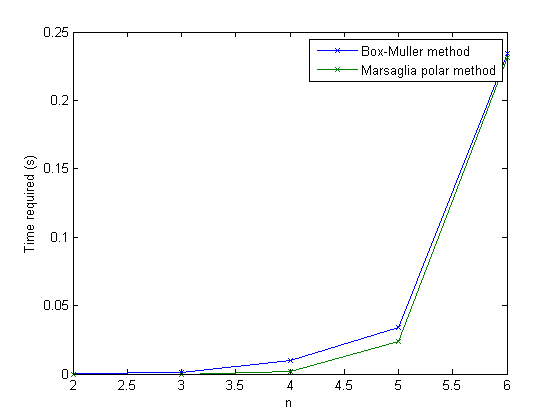
\includegraphics[width=0.5\textwidth]{Q13fig01.png}
\caption{\label{fig:fig01} Plot of elapsed time}
\end{figure}

\end{enumerate}
\end{document}